%
% File hicss51.tex
%
% Contact: Holm Smidt, hsmidt@hawaii.edu
%%
%%
%% Based on the style files for ACL 2015 by 
%% car@ir.hit.edu.cn, gdzhou@suda.edu.cn


\documentclass[10pt]{article}
\usepackage[T1]{fontenc}
\usepackage[latin1]{inputenc}
\usepackage[table]{xcolor} 
\usepackage[letterpaper]{geometry}
\usepackage{hicss51}
\usepackage{times}
\usepackage[none]{hyphenat}
\usepackage{url}
\usepackage{latexsym}
\usepackage{minted}
\usepackage{graphicx}
\graphicspath{{images/}}

\newcommand{\sansserifformat}[1]{\fontfamily{cmss}{ #1}}%

%\setlength\titlebox{5cm}

% You can expand the titlebox if you need extra space
% to show all the authors. Please do not make the titlebox
% smaller than 5cm (the original size).


\title{An Explicative and Predictive Study of Employee Attrition using Tree based Models}

\author{Nesreen El-rayes\\
  MTSM at NJIT \\
  {\underline{nde4@njit.edu}} \\\And
  Michael Smith\\
  MTSM at NJIT \\
  {\underline{mes6@njit.edu}}\\\And 
  Stephen Taylor\\
  MTSM at NJIT \\
  {\underline{smt@njit.edu} (Corr. Auth.)} \\}

\date{}

\begin{document}
\maketitle
\begin{abstract}
We develop tree based models to estimate the probability of an employee leaving a 
firm during a job transition from a dataset of anonymously submitted resumes 
through Glassdoor's online portal.  Dataset  construction and summary 
statistics are first summarized followed by a more in depth examination  
through four exploratory studies.  Insights provided by these studies are then 
used to engineer features that serve as input into subsequent attrition related 
predictive models.  We finally perform a thorough search through several dozen binary 
classification techniques in the cases of an original and extended feature set.  
We find tree based methods including random forests and light gradient boosted trees 
provide the overall strongest predictive performance.  Finally, we summarize ROC curves 
for several such models and describe future potential research directions. 
\end{abstract}

\section{Introduction}
Building and maintaining a stable, productive, collaborative, and high-quality workforce is a primary concern 
of the majority of corporate officers as success in this area tends to be a key contributing factor to the 
overall prosperity of the firm, c.f. \cite{Mir1993} for a survey of relevant issues.
Inevitably, all firms will experience employee attrition.  
Involuntary attrition is often the result of profitability and performance pressures, department or business 
line obsolescence, and mergers and acquisitions, among other factors \cite{Datta2009,Grip2006,SHAU1998}.  In contrast,
voluntary attrition is driven predominately by employee concerns \cite{Singh2012}.  Such considerations 
may focus around, but are not limited to, managerial direction, compensation and benefits, firm culture, 
firm desirability and location, promotion potential as well as non-firm specific motivations, e.g. medical 
conditions or retirement. 
  
A central objective of the majority of human resource departments is to understand the root causes 
behind voluntary employee attrition and develop an associated mitigation strategy.  Effectively 
navigating such issues generally results in explicit positive monetary effects stemming from increased 
firm revenue and cost reductions manifested through the work product of highly performant retained employees. 
In addition, identifying and resolving issues found to be common to employee attrition often implicitly 
enhances firm culture and workplace desirably, which in turn, enables the recruitment of higher quality 
staff who further improve retention, firm operation, and business practices, c.f.  \cite{Cook1986,Free1994}.  
The compounding effect of the employee attrition feedback loop on overall firm
success or failure provides, in our view, the essential motive to 
investigate the issue. 

Traditionally, employee attrition and retention issues tend to examined by qualitative and anecdotal 
measures.  Specifically, human resources staff typically conduct exit interviews after an employee provides 
a resignation notice in order to ascertain the motivations behind the decision to leave \cite{Giac1991}.  Although 
these conversations may be direct and candid, i.e. in the event an employee is leaving for a significantly 
more senior role or needs to change geographic location for family related purposes, in actuality, human resources staff
encounter considerable difficulty discerning the employee's true motivation.  By way of example, employees 
seldom offer negative criticism of management during exit interviews for fear of future personal retribution 
or inadvertent retaliation towards their close colleagues who will still remain at the firm.
These circumstances impact the employee attrition data aggregation and quality assurance process 
by making it cumbersome, at a minimum, which leads to additional difficulties determining which 
attrition issues should be of primary importance for management to resolve. In addition, employee 
attrition data is generally highly confidential and only accessible to key stakeholders internally 
within a firm.  This fact has been a major impediment to the progression of academic research on 
this topic. 

Recently, internet based platforms such as Glassdoor and LinkedIn, which are oriented towards working 
professionals, have amassed large quantities of publicly available information from individual 
employee resumes including employment history, frank reviews of firm culture, desirability, and management
as well as anonymous feedback.  Although this data often lacks attritional motivation information at 
the individual employee level, when combined with aggregate firm culture and management rankings, 
one may glean a number of insights into the collective behavior and motivations behind individual 
decisions to transition to a new employer. Our major aim is precisely in this vein.  More specifically, 
we conduct a quantitative data analysis of employee attrition motivations as well as develop 
predictive models that will enable human resources staff to identify employees whose firm separation 
may be imminent.

The main contributions of this work include an extension of \cite{Smart2016} where the authors 
examine employee 
attrition and retention issues based upon 
a collection of approximately five thousand anonymously submitted resumes to Glassdoor.  
Specifically, we examine industry job transition patterns, independence of company ratings 
provided on the Glassdoor website, and distribution related aspects of these variables 
contained in this dataset.  We further consider how to apply modern binary classification 
methods to predict the likelihood of employee attrition.  In particular, we examine the 
performance of the linear model considered in \cite{Smart2016} against logistic regression, 
decision tree classifiers, and random forests.  We then extend the feature set considered in this 
first student 
and perform a thorough search over dozens of binary classification methods to determine 
the top performers which we find to be tree based models.
 Lastly, we delineate 
future data acquisition, analysis and model development extensions that we seek to investigate 
in future work. Although a few authors have recently approached attrition prediction 
from a modern classification model perspective, i.e. \cite{Fri2018}, we conduct the first 
thorough test of dozens of such models and conclude tree based models offer the strongest 
overall performance from a ROC curve perspective.

This article is organized as follows: In Section \ref{datsec}, we describe the content 
of the job transition dataset being considered and compile a number of 
summary statistics that motivate latter model development.  In Section \ref{datstu},
we pursue a more detailed examination of this dataset by identifying industry transition 
patterns, variable importance related to attrition identification, and 
rating variable independence.  Then in Section \ref{modsec}, we consider several 
models to address the binary classification attrition problem and provide a 
corresponding performance comparison.  Finally, in Section \ref{consec}, we 
summarize our main findings and provide ideas for future extensions of this work.

\section{Data Description and Summary} \label{datsec}

We first turn to describing the content extracted from a collection of 
employee resumes that will form the basis for subsequent attrition studies. 
Next, we provide a variety of summary statistics of this information that 
are relevant for the design of latter predictive models.  Then we discuss 
our data normalization process and 
features constructed from this original data which will be utilized 
as input into these models.

\subsection{Data Source Description}\label{datdes}

We worked in conjunction with the authors of \cite{Smart2016} to obtain 
a collection of 5550 examples of employee job transitions between 
2007 and 2016 which were sourced from an extensive proprietary database of 
resumes shared anonymously though Glassdoor's platform.  A job transition 
is defined to be any instance of an employee listing a new role on their 
resume which may be associated with the current or a new employer
which distinguishes between internal and external moves.  Internal moves are typically 
significant in the sense of the employee either changing roles or 
being promoted within an organization as opposed to being reassigned 
within a current team. External moves are of interest for our 
attrition studies since in this situation employees leave the original 
firm entirely.

We summarize several salient features of the dataset construction process 
and expound upon details relevant to model development below; we refer the
reader to \cite{Smart2016} for a complete description of the data source. 

Each employee job transition contains 45 attributes.  Relevant attributes 
include employee specific information; namely, a binary identifier 
indicating if the employee remained within or left their original firm,
the start and end dates of employment at the original firm, the 
employee's average salary during their tenure with the original employer, 
and the employee's job title. 
In addition, each transition includes employer related information. 
Specifically, employer name and metro location, the industry sector of which the employer 
is a member, the founding year of the firm, and the total number of employees. 
Finally, employer rating information is included.  Particular ratings are 
given for the following Glassdoor created categories: overall, firm CEO, friend recommendation 
business outlook, career opportunities, compensation and benefits, culture and values, 
worklife balance, and senior management performance. 
We note that in the event the employee transitioned to a new firm, when applicable,
the above information specific to both the original and new employer is present in this dataset. 
Finally, this dataset if fully populated with the exception of missing values in 
approximately 6\% of the original and new employer founding year values, respectively;
such null values are disregarded 
only in studies that depend upon this variable below.

\subsection{Summary Statistics, Feature Engineering and Data Normalization}

First, several summary statistics are presented in order to outline 
the main content of the dataset that will be further explored below.
Next, we discuss our feature construction process to build inputs 
that will be important to latter exploratory studies and predictive 
model design.  Finally, we describe the quantile normalization process 
that is utilized in order to ensure all variables are on the same scale prior 
to being input into the predictive models.

Of the 5550 total employee job transitions in this dataset, 
a total of 1429 employees remained at their present firm whereas a majority of 4121 
transitioned to a new firm.  This confirms a claim \cite{Smart2016} indicating 
that approximately three quarters of employees leave their employer during a job 
transition.  We now graphically summarize several distributional aspects of 
attributes associated with these transitions.

Compensation, benefits, and other forms of financial remuneration typically play 
a critical role in an employee's job transition decision process.  In fact, an offer to 
substantially increase one's salary is a common impetus for a job transition. 
In the left subplot of Figure \ref{fig:avgsal}, we plot the average 
annual salary distribution 
of the employer during their tenure at their original employer over our full dataset.  
Salaries ranged from \$15,140 to \$240,000 per year.  We note that this sample 
is slightly overweight in terms of the representation of low-wage workers 
in comparison with national income distributions as compiled 
by the Bureau of Labor and Statistics May 2018 National Occupational 
Employment and Wage Estimates. In addition, 
approximately 9\% of workers have salaries greater than \$100,000, which further 
indicates a slight low-wage bias with respect to the entire United States workforce population. 
However, we note the generate shape of this distribution does indeed closely approximate 
that of the full workforce.
%
\begin{figure}[thb]
    \centering
	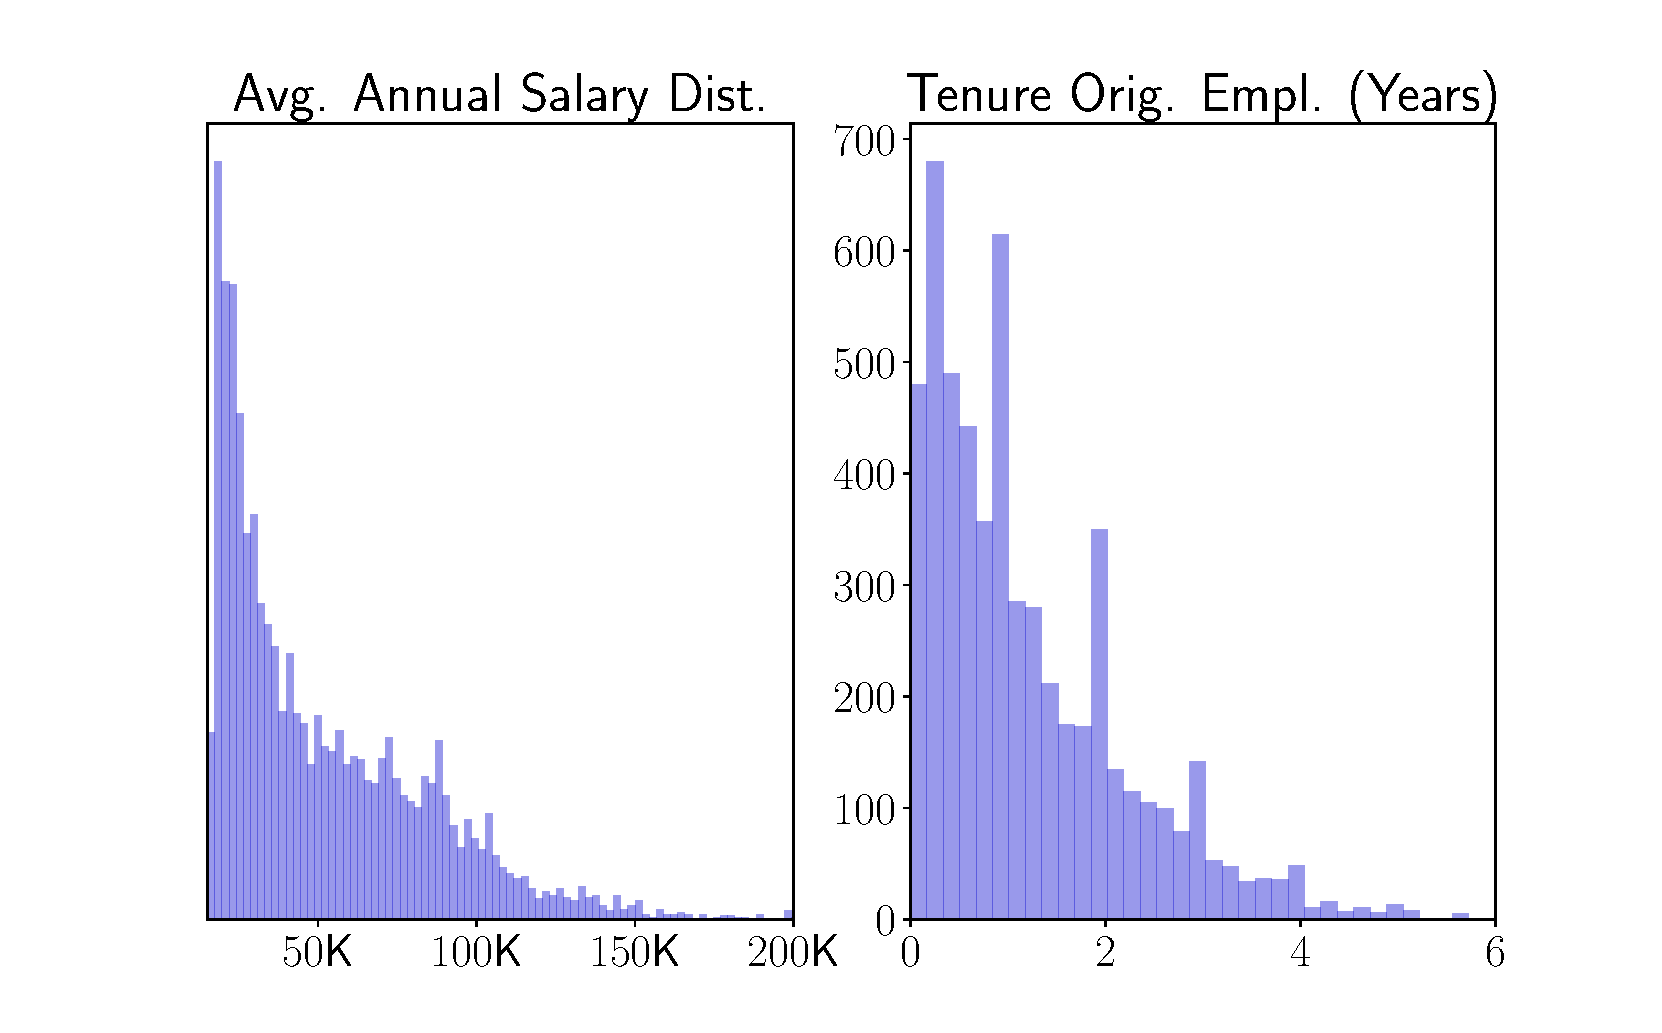
\includegraphics[width=1.0\linewidth]{avgsal.pdf}
    %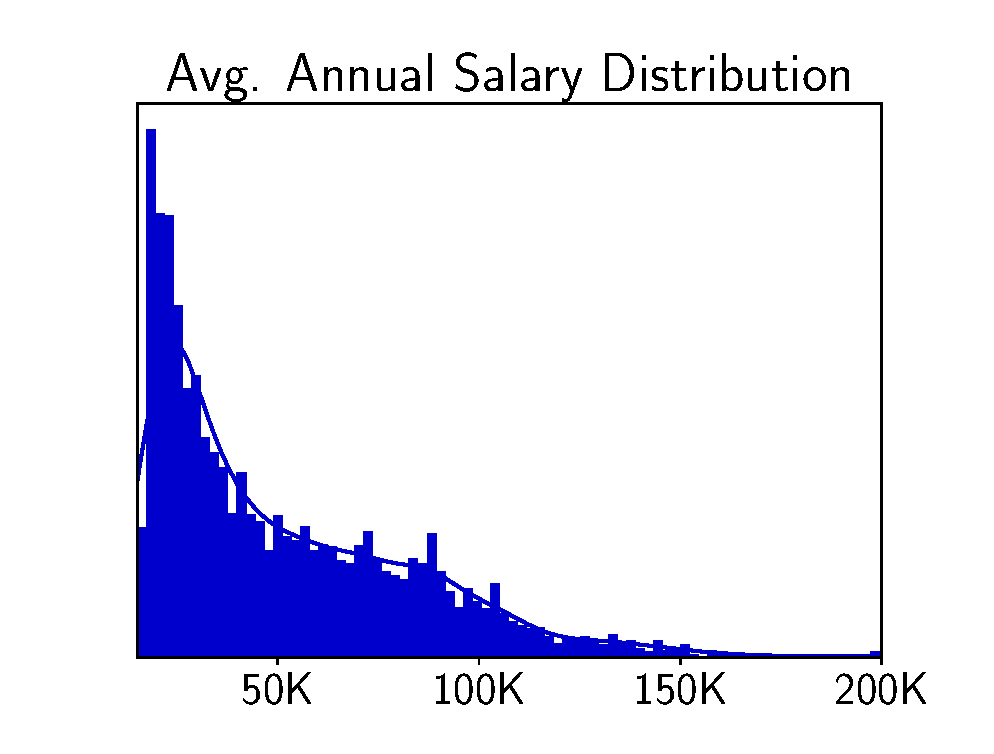
\includegraphics[trim={3cm 3cm 3cm 3cm}, clip,width=0.9\linewidth]{avgsal.eps}
	\caption{Employee average salary and tenure distribution at original employer}
	\label{fig:avgsal}
\end{figure}
%
In the right subplot of Figure \ref{fig:avgsal}, we display the tenure of each 
employee at their original employer prior to a job transition which is similar to
summary information presented in \cite{Smart2016}. Note that overall these tenures 
are relatively short and the distribution exhibits concentrated counts near end of year 
times when performance reviews typically take place.  

Next, in Table \ref{tab:indtab}, we count the industry of the original employer 
of all job transitions being considered and display all such industries exceeding 
50 transitions.
%
\begin{table}
  \rowcolors{2}{gray!25}{white}
  \centering
  \caption{Job Transition Counts Per Industry}
  \begin{tabular}{cccc}
    \rowcolor{gray!50}
      Industry & Count & Industry & Count \\
      Retail & 1357 & Manufact. & 191\\
      Education & 766 & Insurance & 144\\
      Info. Tech. & 718 & Media & 113\\
      Finance & 590 & Acct. \& Legal & 101\\
      Bus. Services & 369 & Energy & 92\\
      Food Services & 275  & Travel & 70\\
      Telecom & 248 & Biotech & 62\\
      Health Care & 208 & Transportation & 58\\
	\label{tab:indtab}
  \end{tabular}
Original employer sector counts for industries with more than 50 job transitions.
\end{table}
%
Note that the Retail and Education industries are overrepresented which 
provides a further indication as to why this dataset includes a higher occurrence 
of lower salaries  than the full national wage distribution. In addition, we have sufficient data to study employee industry 
transition patterns for many of the industries listed in this table which 
we explore in more detail in the subsequent section.

In Figure \ref{fig:emplstat}, we display two additional histograms related to original 
employer specific information.  In the left subplot, we present the distribution of the 
original firm's founding date.  This histogram was left truncated to begin at 1750 with a minimum 
founding date of 1625 for the City of New York.  Typically, firms with earlier founding 
dates are municipalities or governmental organizations. 
%
\begin{figure}[thb]
    \centering
	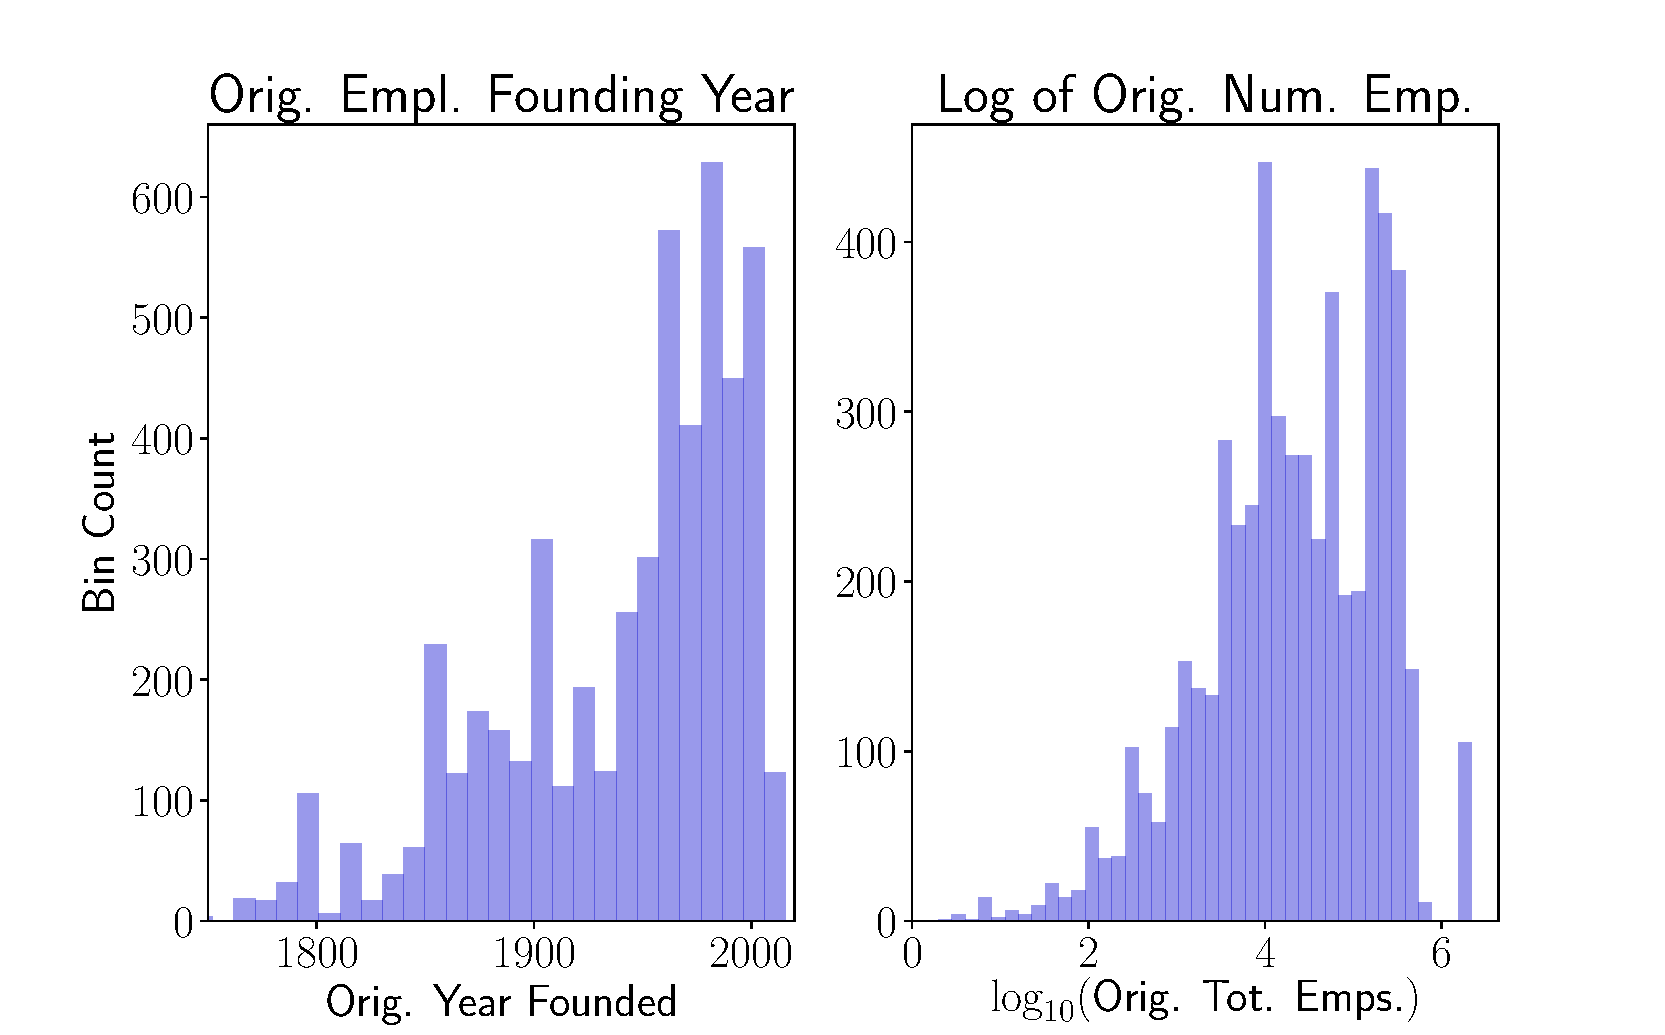
\includegraphics[width=1.0\linewidth]{emplstat.pdf}
    %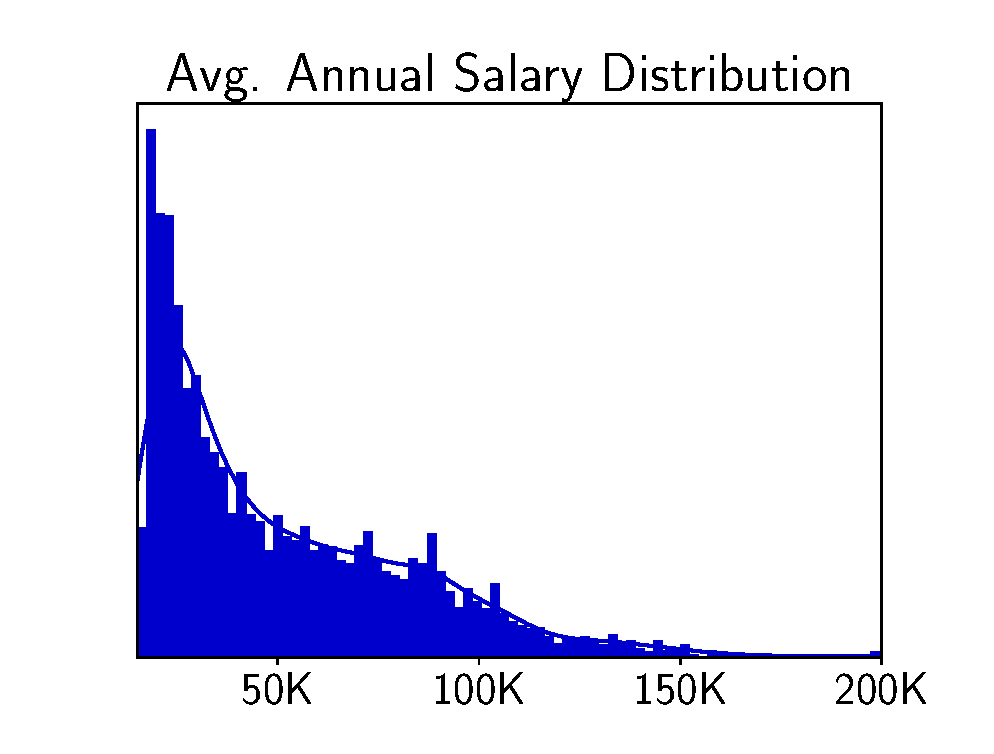
\includegraphics[trim={3cm 3cm 3cm 3cm}, clip,width=0.9\linewidth]{avgsal.eps}
	\caption{Original employer founding year and employee number distributions}
	\label{fig:emplstat}
\end{figure}
%
Note that we have an effective sampling of older and modern firms with a 
median founding date of 1962.  In addition, we consider relatively few 
firms that were founded within the past twenty years in this sample as 
indicated by the height of the final bar of the histogram.   Next, in 
the right subplot of Figure \ref{fig:emplstat}, we display the log-histogram 
of the number of employees at each original firm being considered. The majority 
of employees work at larger firms which employ between ten thousand to one million 
people.  In particular, only a small fraction of employees work at small 
firms with fewer than one hundred colleagues.  Finally, the largest employer 
is Walmart with approximately 2.2 million employees.

Next, in Figure \ref{fig:vioplt}, we display original employer violin plots of ratings data in nine 
categories presented for evaluation on Glassdoor's website which include career opportunities, compensation and benefits, company culture, 
overall rating, senior management, work-life balance, outlook, CEO performance, and friend recommendation 
ratings.  Here mean values are depicted by white circles within each form whereas standard deviations 
about either side of the mean are displayed by centered black bars.  The general shape of 
each violin is determined by a symmetric display of a kernel density estimate of the 
probability distribution of each rating variable.
%
\begin{figure}[thb]
    \centering
	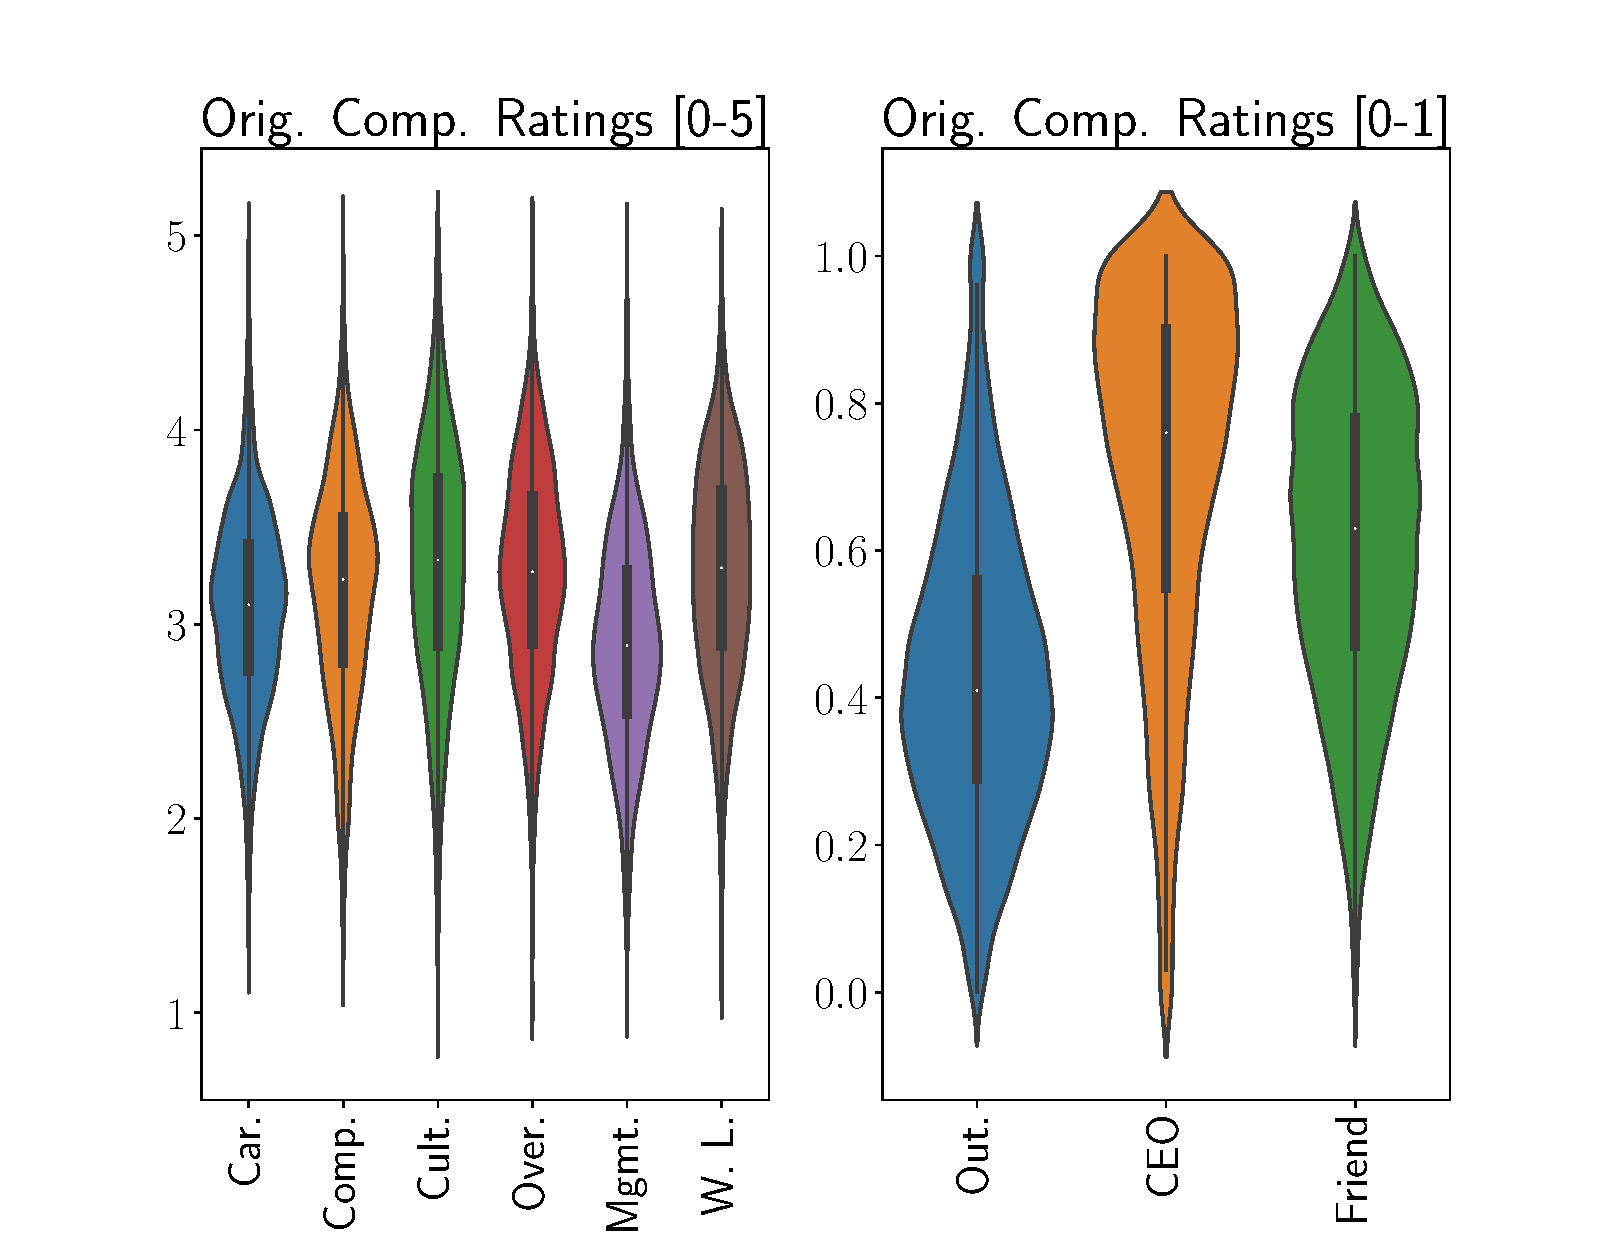
\includegraphics[width=1.0\linewidth]{vioplt.pdf}
    %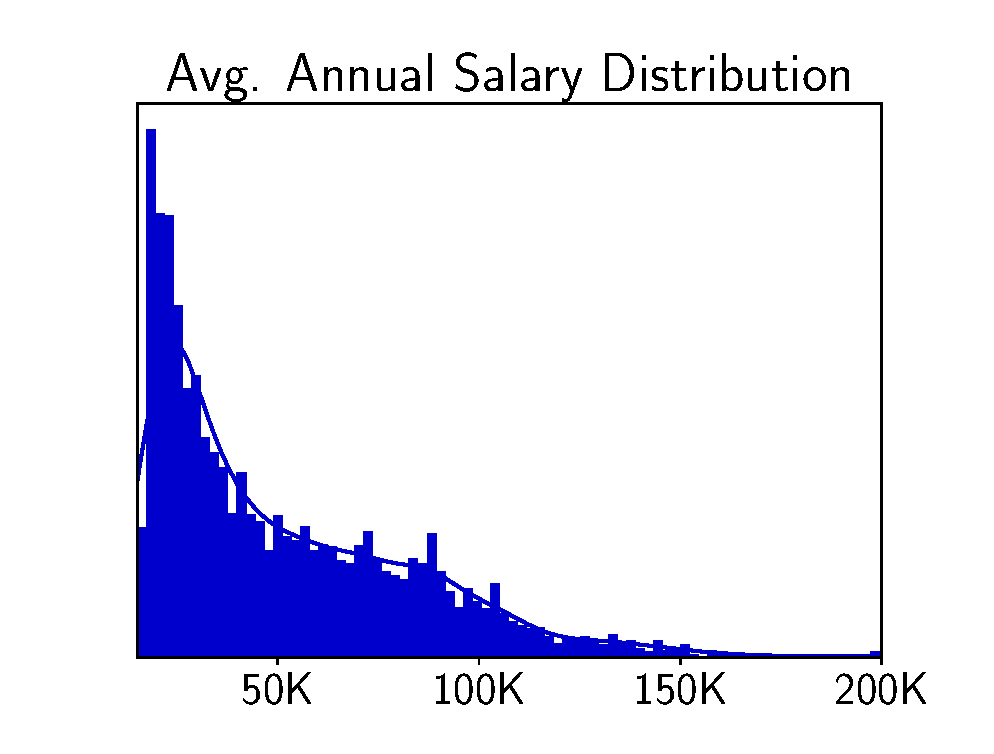
\includegraphics[trim={3cm 3cm 3cm 3cm}, clip,width=0.9\linewidth]{avgsal.eps}
	\caption{Violin plots of original employer ratings information sourced from Glassdoor reviews }
	\label{fig:vioplt}
\end{figure}
%
Ratings with values in the $[0,5]$ range are plotted in the left subplot and those between 
$[0,1]$ are plotted in the right.  We note that no actual ratings fall outside these 
bounds; the slight graphical extensions beyond the boundaries in the plot are due to 
artifacts of the kernel density estimation procedure required to 
produce the visualization and are not representative of the true data. 
In addition, note that one can see management ratings tend to be lower overall than 
other related ratings in the left subplot.  In addition, cultural ratings exhibit 
the greatest dispersion, whereas career ratings are comparatively concentrated.
The distributions of $[0,1]$ valued ratings vary considerably.  In particular, the CEO rating distribution 
is concentrated to the right of the mean largely to a high occurrence of maximum ratings in 
approximately 9\% of the data.  In contrast, company outlook ratings are right-skewed with 
a mean below the average score of 0.5.  Both are less dispersed than the friend recommendation 
rating distribution that also is slightly oriented towards the positive side.

We now describe several elementary features that we construct from the original data that 
will be useful in the below exploratory and predictive studies.  In particular, we will 
consider the percentage salary increase after a transition has been made. 
In addition, we will consider quantile normalized absolute changes in each rating 
category below, e.g. if an employee moved from a 75\%-tile overall rating employer 
to an 85\%-tile, we will save the 10\%-ile difference as a feature.  We feel that these 
features are partially reflective of the thought process of an employee who typically leaves an organization 
for higher salary and improved company culture based on the relative rather than absolute 
differences in these variables, and thus include them as features.  We finally note that 
all variables are quantile normalized in our predictive model studies so as not to bias 
methods due to scaling effects.

\section{Exploratory Insights} \label{datstu}

Now we describe a number of findings originating from the results of an exploratory analysis of 
the job transition dataset which go beyond the level of summary statistics.  In particular, 
we examine to what extent salary increases motivate job transitions.  In addition, if employees decide to 
change industry, we study which industries they are most likely to move towards conditioned 
on their original industry.  We then 
identify which variables when partitioned into employees that remained or left their 
firm differ the most from a distributional perspective to gain intuition on what 
factors should be most important for subsequent model development.  Finally, 
we investigate to what degree the nine rating categories are dependent and 
compute the effective dimension of these variables.

\subsection{Job Transition Salary Changes}
An opportunity to earn a greater salary is often described as a primary motivation 
for a job transition.  We seek to investigate this from a quantitative perspective, 
and first note that approximately 
13\% of transitions occurred without a change in salary. 
In Table \ref{fig:salgr}, we display relative (percentage increase/decrease) and  
absolute salary changes. 
%
\begin{figure}[thb]
    \centering
    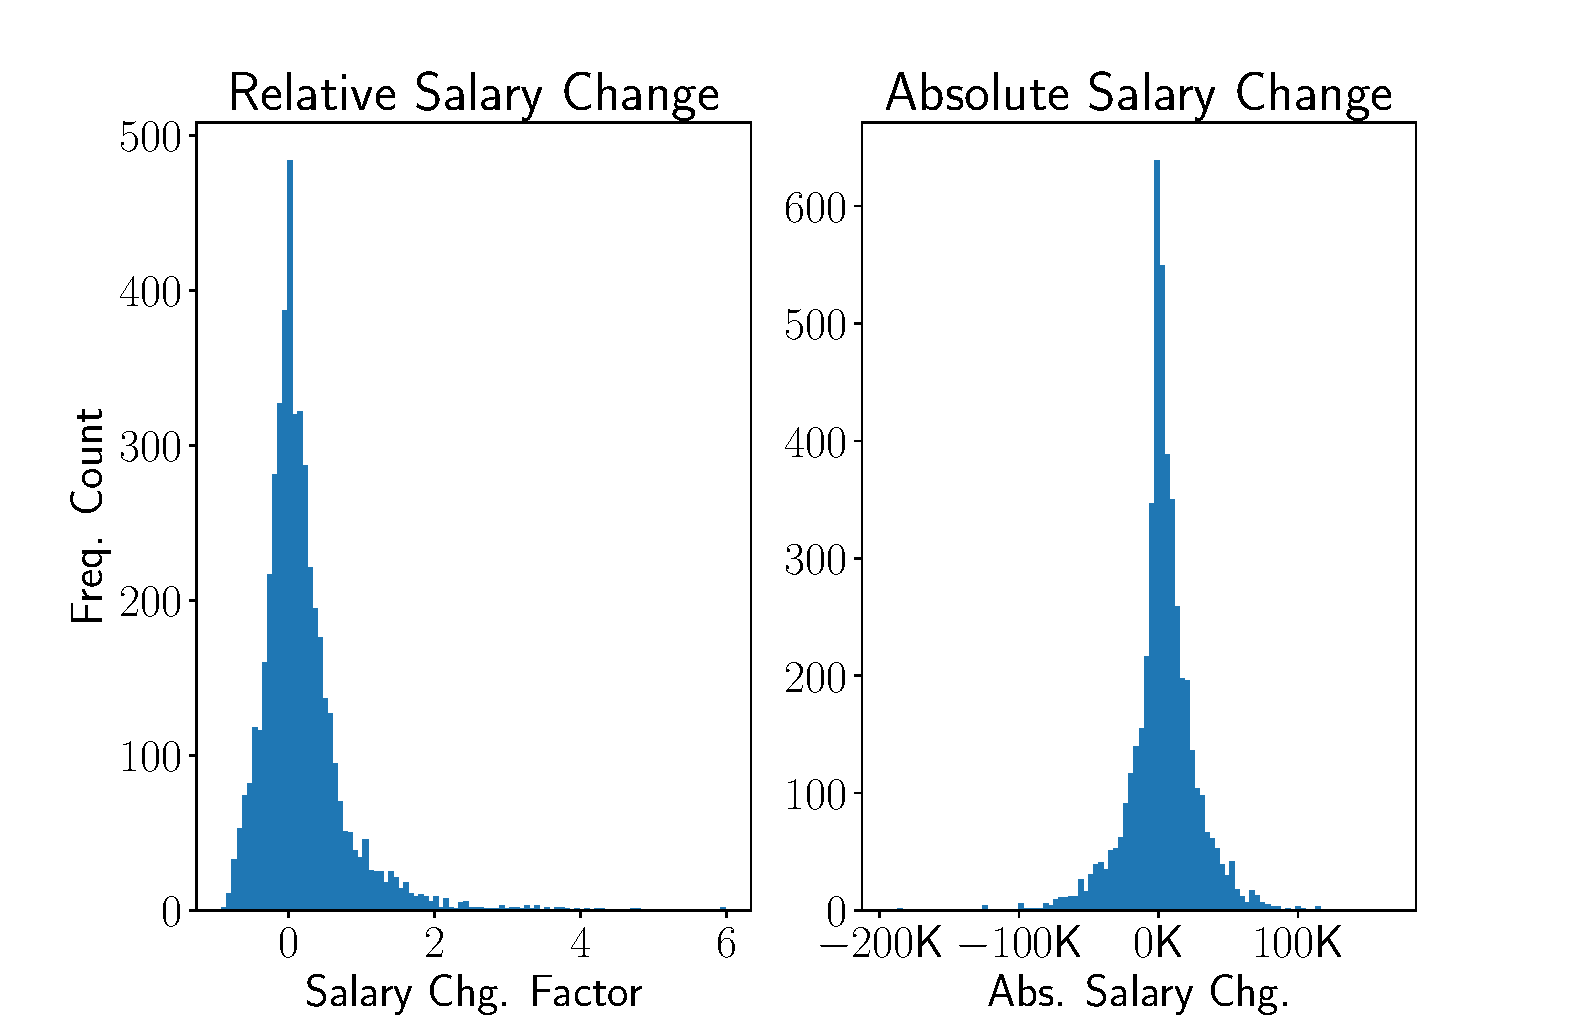
\includegraphics[width=1.0\linewidth]{salgr.pdf}
    %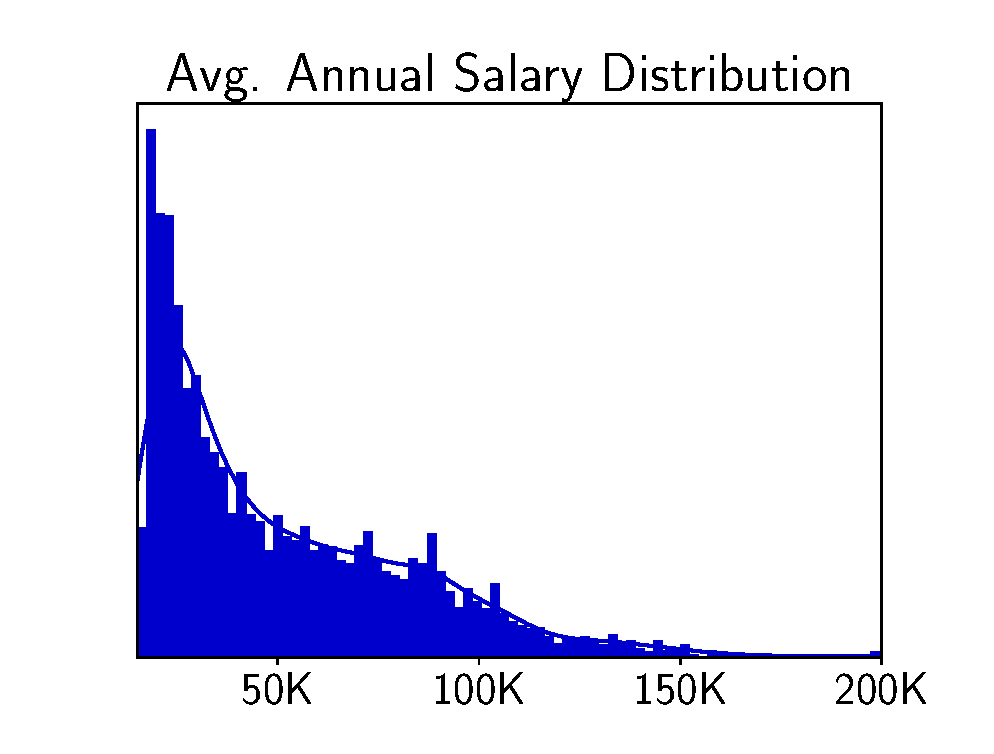
\includegraphics[trim={3cm 3cm 3cm 3cm}, clip,width=0.9\linewidth]{avgsal.eps}
	\caption{Relative and absolute salary differences after a job transition}
	\label{fig:salgr}
\end{figure}
%
First note that this example illustrates the need for considering 
features such as relative salary change since the asymmetry of the relative change salary distribution is 
prominent whereas this is not as clear in the absolute change plot.  
Second, note that there is a wide range of magnitudes of relative salary changes.  In particular, 
approximately 5\% of employees received a salary increase of more than 150\%.  In 
addition, 36\% took a reduction in salary as a part of their transition.  However, the remainder 
received a salary increase which was in many cases quite substantial. 

In the extreme case, one employee transitioned from a teaching assistant to 
education Director at Michigan State University and received approximately a 6X 
salary increase.  In the opposite direction, one employee transitioned from a \$230,000 
salary as a Managing Director in the Education industry to a Logistics Coordinator 
with a \$43,600 annual salary. 

\subsection{Industry Transition Patterns}

Next, we examine how employers either choose to move to a new industry or remain
in that of their original firm as a consequence of their job transition.  
In Figure \ref{fig:transmat}, we display a heatmap of the percentage of 
employees that started in an industry indicated by the lower column labels and 
transitioned into the industry in the row labels. 
%
\begin{figure}[thb]
    \centering
	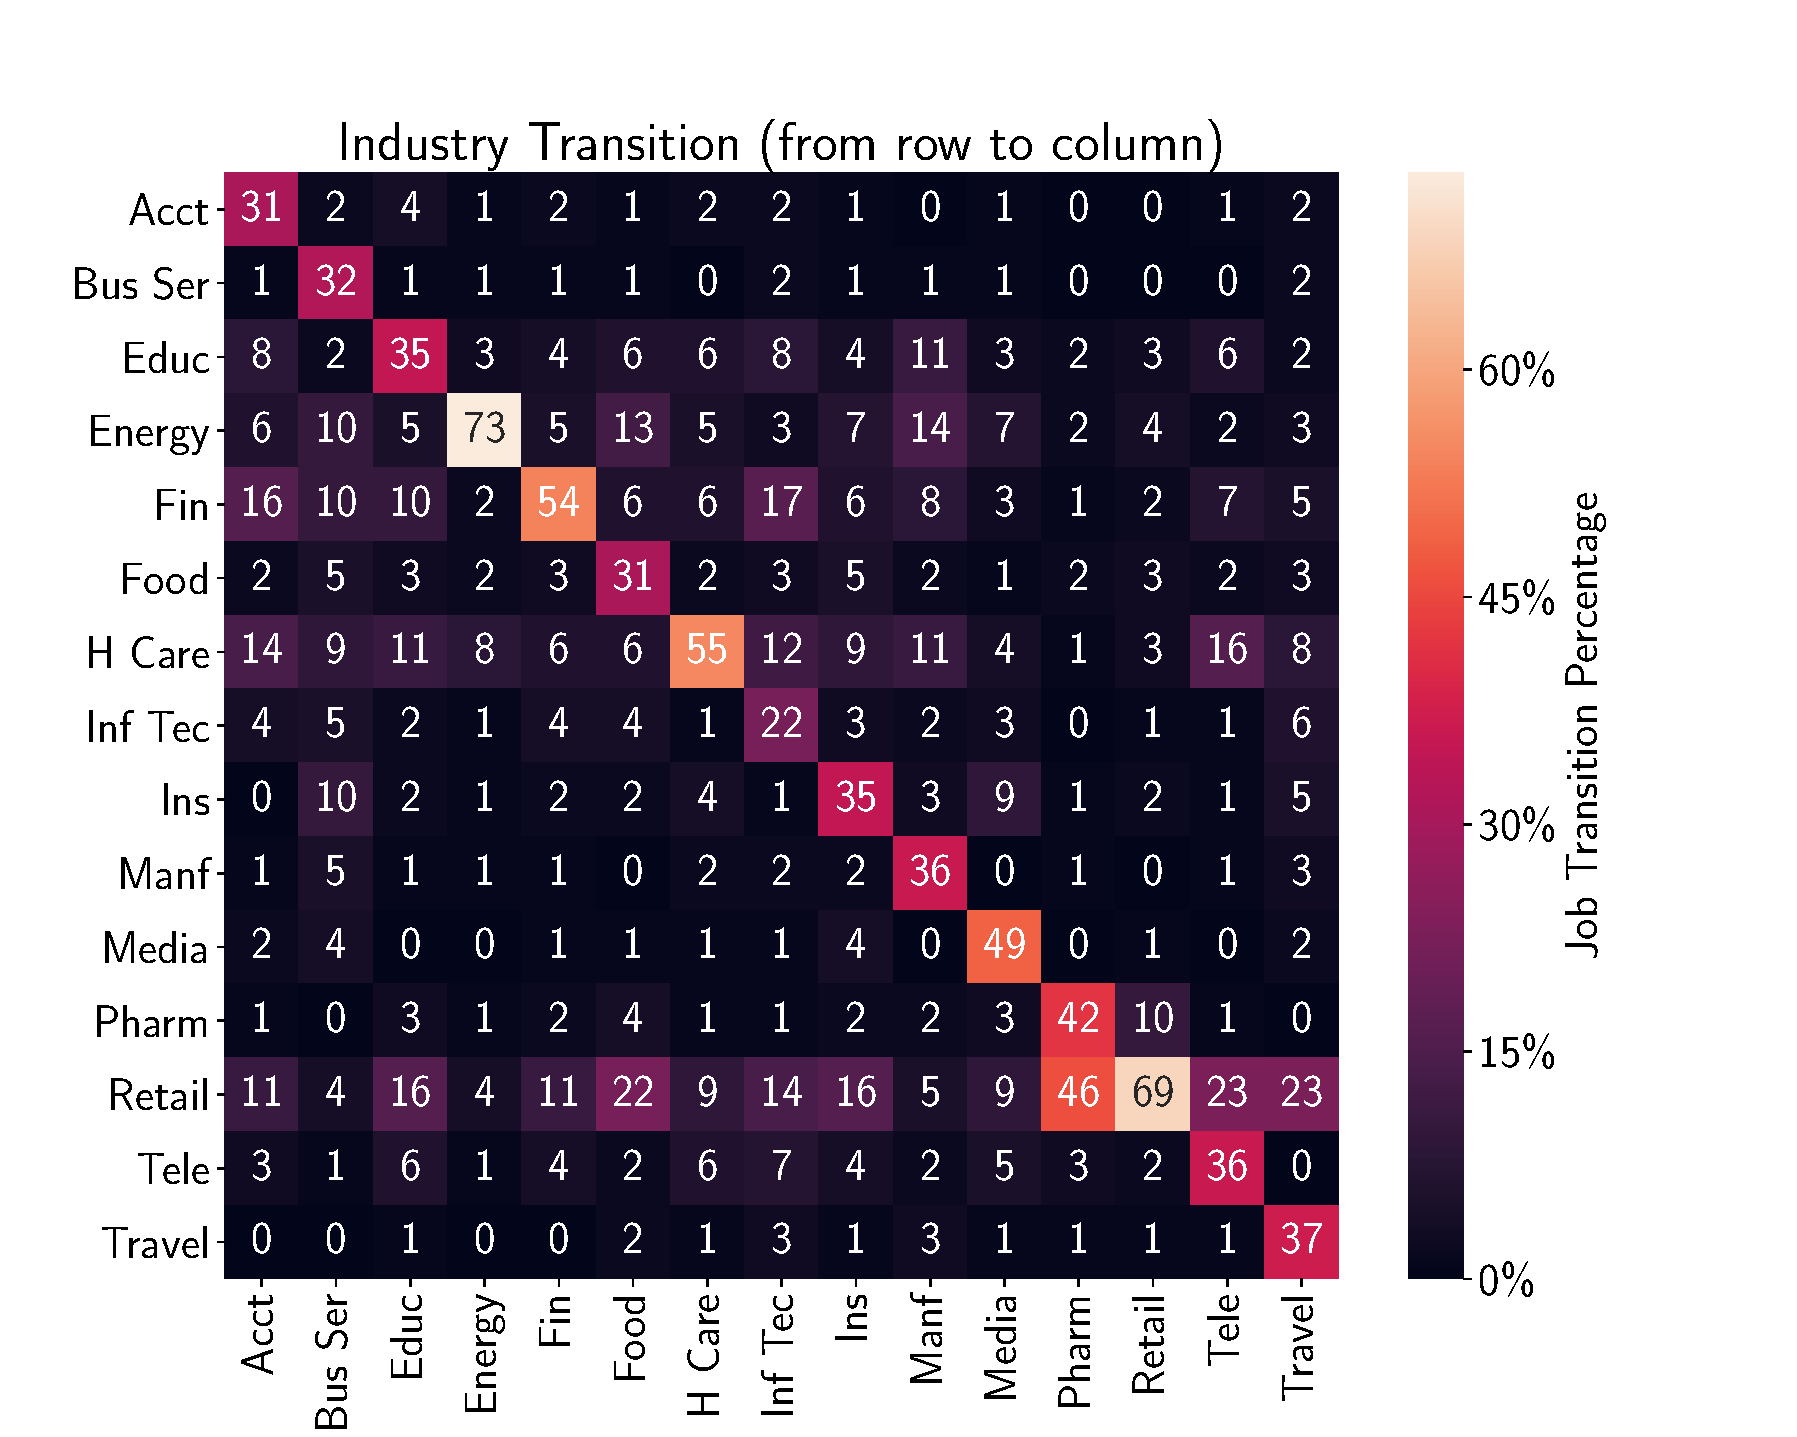
\includegraphics[width=1.0\linewidth]{transmat.pdf}
    %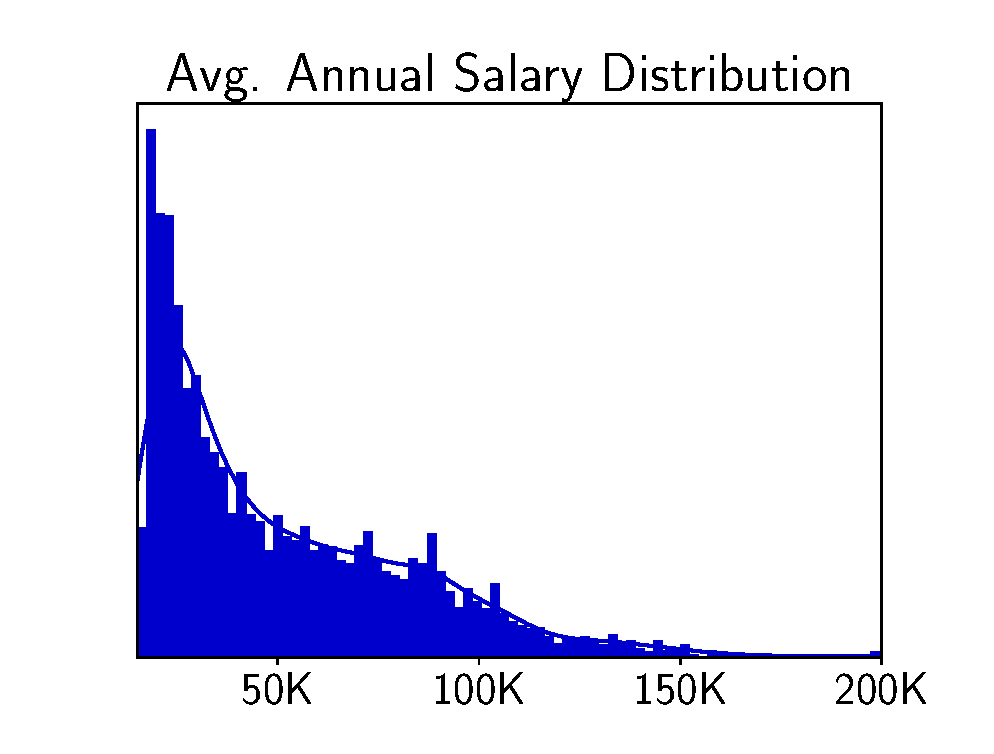
\includegraphics[trim={3cm 3cm 3cm 3cm}, clip,width=0.9\linewidth]{avgsal.eps}
	\caption{Industry transition percentage: original firm 
   industry given in columns and new/same in rows}
	\label{fig:transmat}
\end{figure}
%
Note that both the energy and retail industries tend to retain a considerably 
greater proportion of their employees than the others.  An interesting example 
along these lines is the Pharmaceutical industry of which 46\% of employees 
transition to the retail industry while only 42\% remain; this is the only industry in which 
a greater percentage of employees transition to another industry rather than 
remain in the original.  Moreover, the information technology industry has 
the lowest retention rate with more than half of transitions out of this industry 
going to the financial, health care, retail, and education sectors.  This is understandable 
due to the skill requirement prevalence of IT positions across all these industries.  
Finally, we note that the retail industry is the most popular industry to transition 
into overall from a different original industry.

\subsection{Attrition Identification Variable Importance}

Now, we separate the job transition  dataset into a retention subset 
where employees remained with their current employer, and an attrition set for those who 
choose to find a new employer. We compare the distributions of all 
numerical variables available for both groups 
in order to identify which variables have the most distinct 
distributions.  In Figure \ref{fig:discdist}, we display the 
distributions of the original firm friend recommendation and 
worklife balance rating variables for employees who 
stayed with their original firm (green) or transitioned to a new one (red). 
%
\begin{figure}[thb]
    \centering
	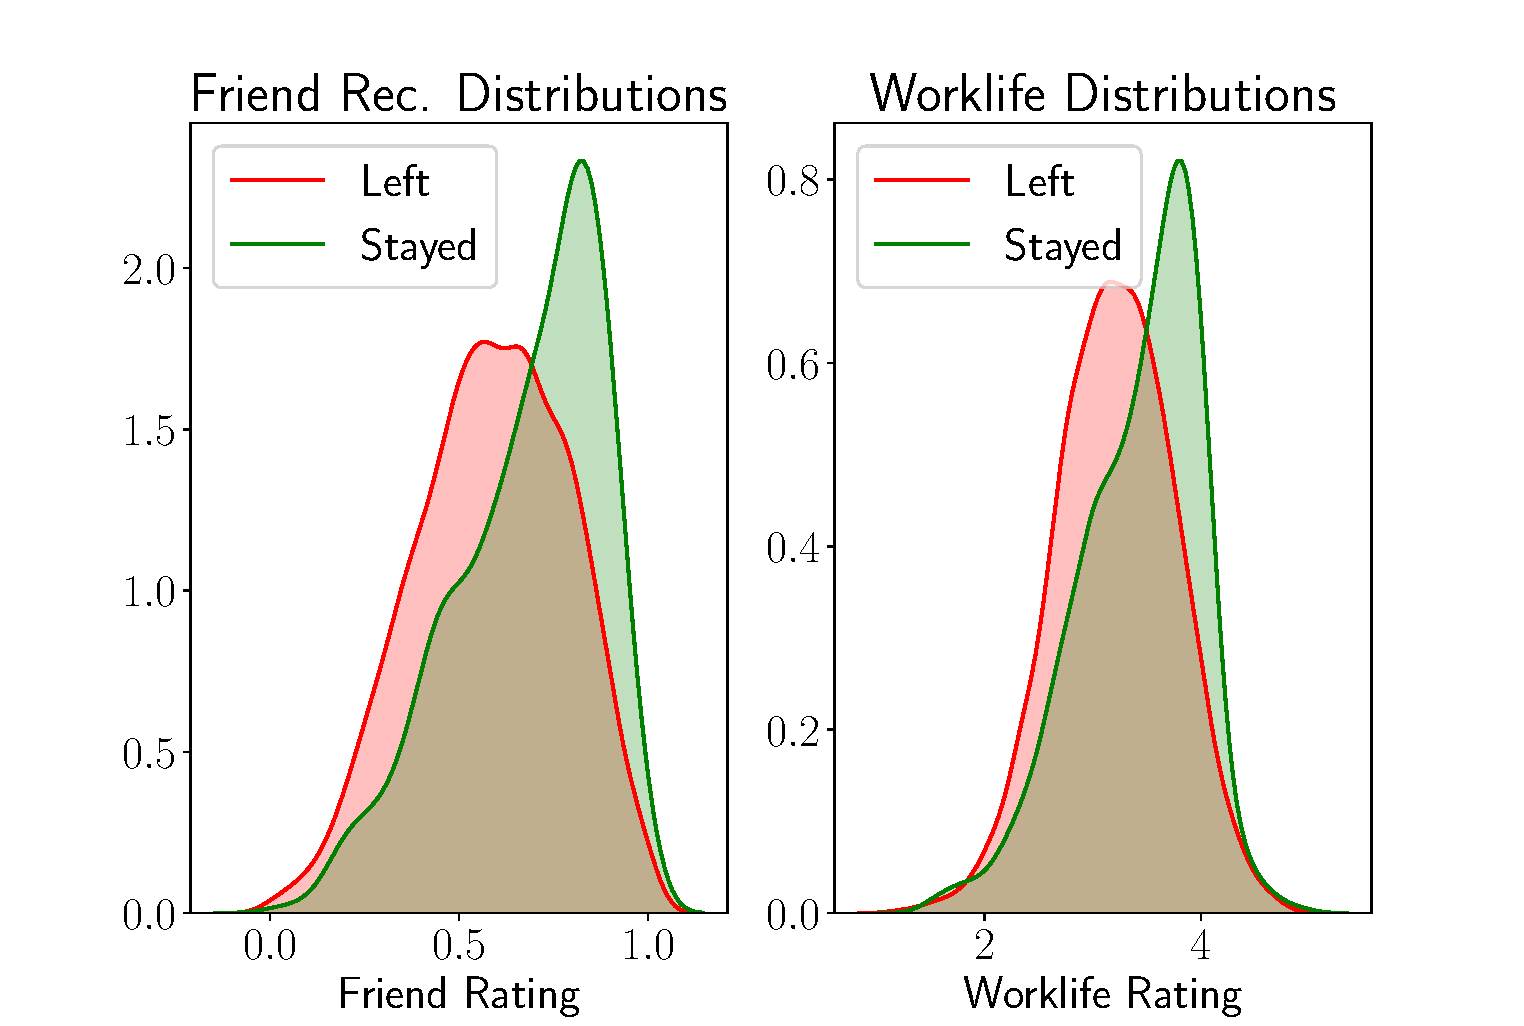
\includegraphics[width=1.0\linewidth]{discdist.pdf}
    %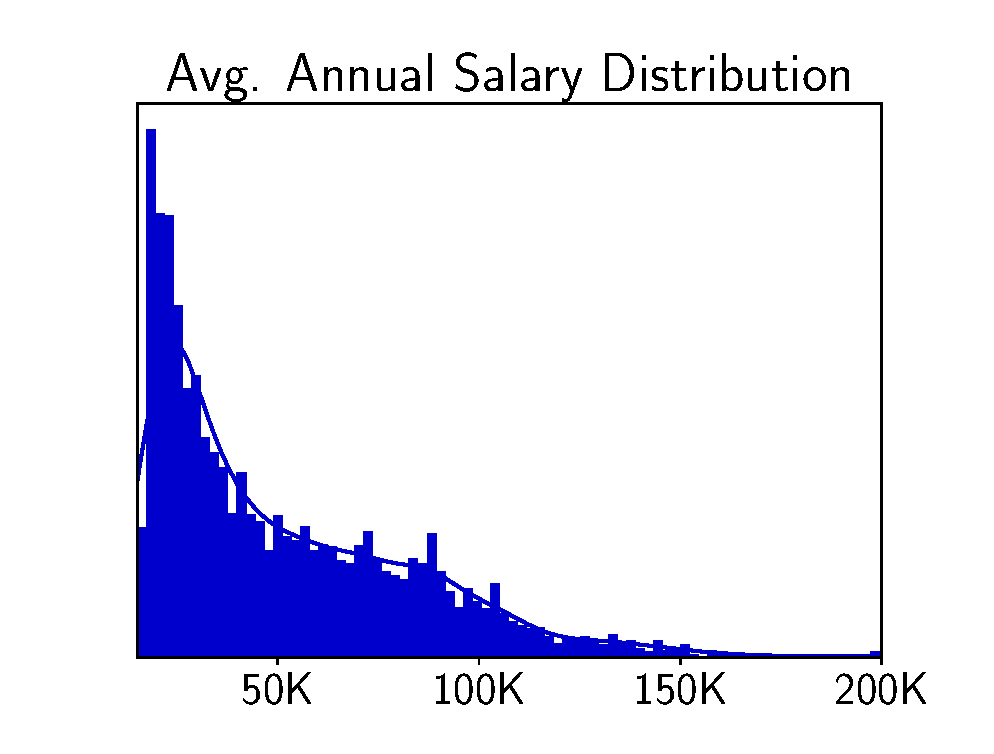
\includegraphics[trim={3cm 3cm 3cm 3cm}, clip,width=0.9\linewidth]{avgsal.eps}
	\caption{Friend recommendation and worklife rating distribution for internal 
    and external transitions}
	\label{fig:discdist}
\end{figure}
%
In addition, we note that the cultural rating distributions exhibited a similar 
although less pronounced behavior.  This provides an indication that both 
these variables will be of importance when attempting to discriminate between 
the two groups in our latter predictive studies. 

\subsection{Firm Ratings Principal Components}\label{pcasec}

When users fill out Glassdoor surveys that ultimately determine the 
company ratings provided in the job transition dataset, they are asked to 
rate a firm in the nine categories described in Section \ref{datdes}.
It is natural to allows one's overall view on the firm influence 
the manner in which ratings are assigned for each of these
categories, i.e. they are not necessarily independent.  We will 
conduct a principal component analysis on a quantile normalized 
version the full original ratings dataset of nine categories in 
order to ascertain the effective dimensionality of this information. 

Specifically, let $r_i^j$ for $i=1,\ldots,n=5550$ and $j=1,\ldots,9$ denote 
the $i$ ratings available for $j$ categories. Consider the sample covariance 
estimator of the quantile normalized ratings data
%
\begin{equation}
    \hat{\Sigma} = \frac{1}{n-1}\sum_{i=1}^n (r_i^j-\bar{r}^j)(r_i^j-\bar{r}^j)^T, 
\end{equation}
%
where here $\bar{r}^j$ denotes the mean value of the $j$-th variable.  Then, we 
perform an eigen-decomposition 
%
\begin{equation}
    \hat{\Sigma} = Q\Lambda Q^{-1}
\end{equation}
%
where here the $i$-th vector of $Q$ is the $i$-th eigenvector of $\hat{\Sigma}$ with 
corresponding eigenvalue $\lambda_i$ which is the $(i,i)$ entry of the diagonal matrix 
$\Lambda$.  This decomposition holds since $\hat{\Sigma}$ is assumed to be positive 
definite, and in addition, we take an ordering $\lambda_1\geq\lambda_2\geq \ldots\geq \lambda_9$,
c. f. \cite{Shlens05atutorial} for an overview of principal component analysis.

In the left subplot of Figure \ref{fig:pcagr}, we display a heatmap of the 
original employer ranking correlation matrix.  Note that all pairs 
generally exhibit high correlation which demonstrates 
that it is necessary to account for the dependency structure of the ranking 
variables.  In the left subplot, we display the percentage variance explained curve 
whose values are defined to be $w_i = \sum_{j=1}^i\lambda_i/\sum_{j=1}^9\lambda_j$. 
%
\begin{figure}[thb]
    \centering
	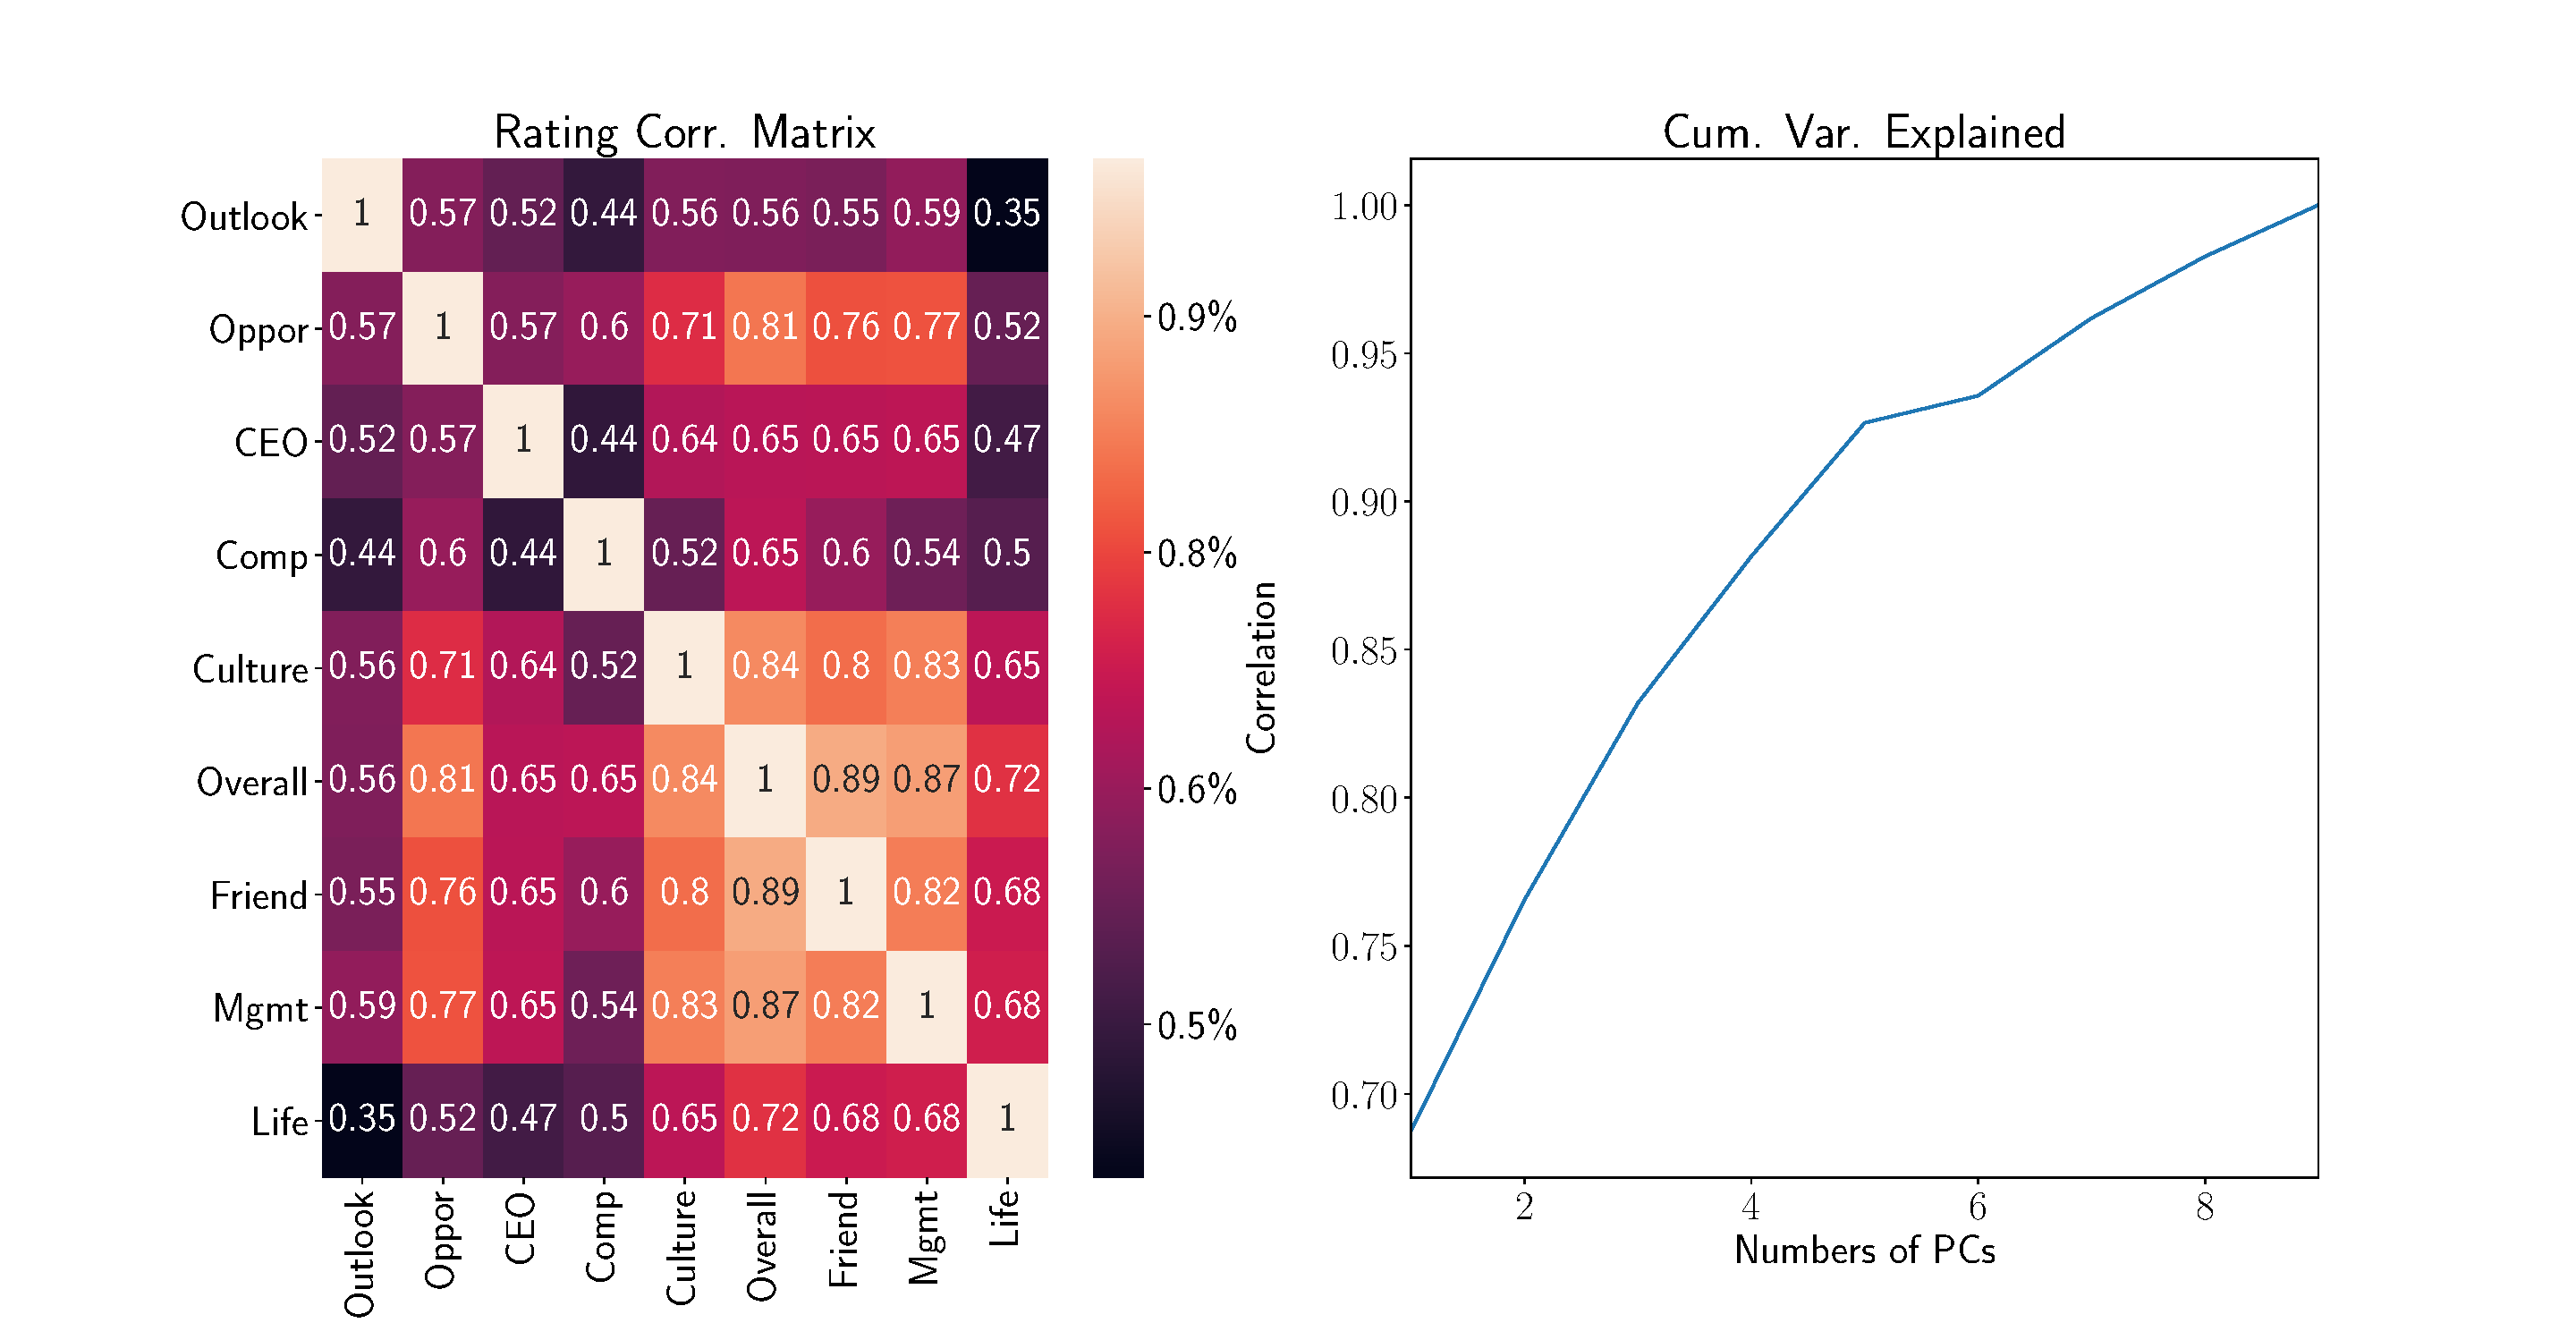
\includegraphics[width=1.0\linewidth]{pcagr.pdf}
    %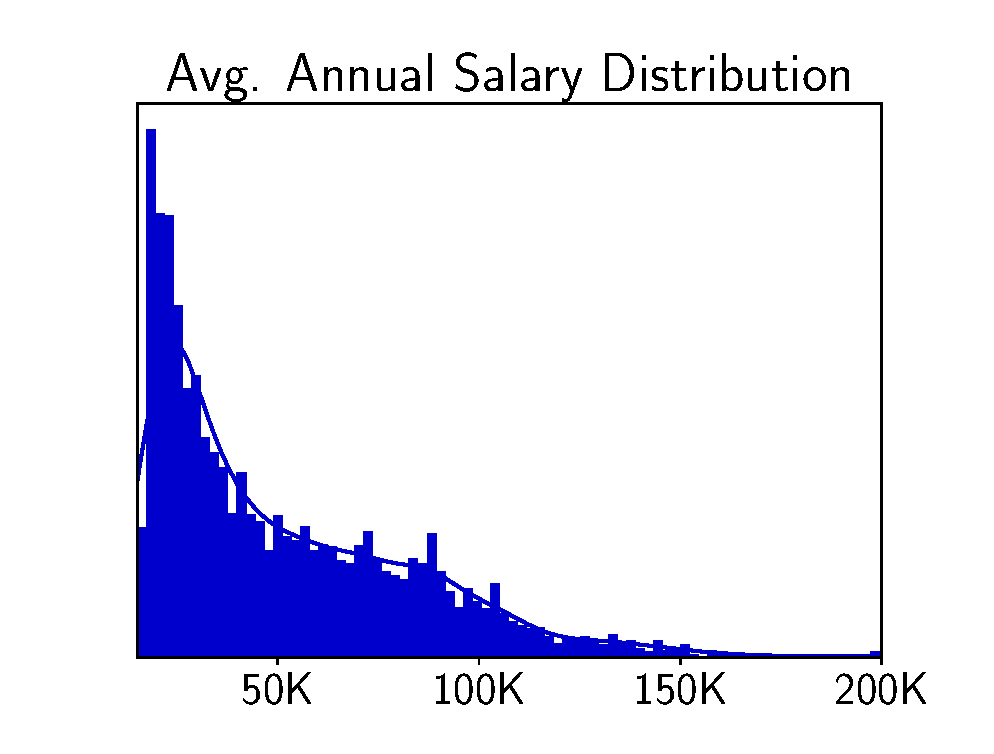
\includegraphics[trim={3cm 3cm 3cm 3cm}, clip,width=0.9\linewidth]{avgsal.eps}
	\caption{Original employer ranking correlation matrix and percentage variance 
    explained curve}
	\label{fig:pcagr}
\end{figure}
%
The first principal component contains just under 70\% of the variation of the data 
and is given in normalized form by  
%
\begin{equation}
    q_1 = [0.27,0.34,0.30,0.28,0.36,0.38,0.37,0.37,0.30] 
\end{equation}
%
which is near a uniform weighted average of the rankings with additional 
weight placed on career opportunities, overall rating, friend recommendation, and 
senior management rankings. In addition, the percentage variance explained 
gradually increases to approximately 92\% at five principal components and 
there is no clear separation between the signal and noise portions of this data.
We conclude that it will be useful to include the quantile normalized 
ranking weighted average in our subsequent predictive studies, but we 
also retain all ratings variables given these percentage variance explained results. 

\section{Towards an Attrition Model}\label{modsec}

We now focus on extending beyond the prior exploratory data analysis and systematically construct 
a series of refined models to predict whether an employee will remain with their original employer or 
leave for another firm during a job transition.  We consider two datasets below first 
consisting of the original variables considered in \cite{Smart2016} and then an extended 
version which includes additional features further described below. Initially we 
consider simple linear and logistic regression and decision tree classifiers to establish 
baseline results.  We then more systematically search through several dozen binary classification 
methods to identify which have the strongest performance from an ROC curve perspective.  We find 
that tree based models tend to be identified in this regard and discuss the top performers 
in detail below. 

In all models considered below, we uniformly randomly partition our dataset into 80\% training data 
and 20\% test data.  All models are trained using 5-fold cross validation and all performance 
results are based on evaluation of each model on the test set.  Moreover, each model 
was only ran on the test set a single time. 

\subsection{Linear Review}
First, we recall the linear model in \cite{Smart2016} where the authors fit a linear model 
%
\begin{equation} 
    y = \beta^Tx + \epsilon 
\end{equation} 
% 
where here $\beta = (\beta_0,\ldots,\beta_m)$ and $x=(1,x_1,\ldots,x_{n})$. The 
target variable $y$ is interpreted a probability of leaving their employer and 
$x_i$ denote normalized versions of the ratings, salary, job length, and 
associated control variables including the employee's industry and job title, original 
employer's metro area.

This model is fit in the usual fashion through 
%
\begin{equation}
    \hat{\beta} = (x^Tx)^{-1}x^Ty
\end{equation}
%
which produces a decision function for each job transition from which we may classify 
each as more probably to remain or leave their current employer; here predicted probabilities 
are capped at 1 and floored at 0. Note that the variables 
that are utilized within this model only depend upon information related to the employee's 
current employer which is often the only information that Human Resources staff have 
readily available.  We implement this model and use it as a baseline for comparison against the other
binary classifers considered below. 

\subsection{Logistic Regression} We next extend to a logistic regression model with the 
same variables as the linear model which 
is more suitable for probability prediction and more specifically binary classification 
problems.   In particular, we fit the model 
%
\begin{equation}
    y = (1+\exp(-\beta^Tx))^{-1}.
\end{equation}
% 
where here again the target $y$ represents the probability of leaving the firm. 
Note know that $y\in[0,1]$ which are appropriate bonds for a probability.  This 
model is fit to our data through maximum likelihood estimation. 

\subsection{Decision Tree Classifier}  Next, we explored a variety of additional 
binary classification models utilizing one original employer variables described above.
In particular, we examined quadratic discriminant based classifers, support vector classifiers, 
and tree based methods, among a variety of other techniques.  We found that decision 
trees provided the strongest predictive performance relative to model complexity. 
In particular, if we significantly increase model complexity, we can marginally outperform 
a decision tree classifer; however, it is likely such gains are not meaningful and 
a result of implicit overfitting. 


When constructing decision tree models, we explored trees with depths from 2 to 10 and 
found that depth 5 trees has the strongest overall performance from an area under their 
associated ROC curves. 
A decision tree is fit to the attrition data by using a greedy technique of 
iteratively determining which feature and threshold minimizes performance error 
at each level of the tree.  This method is iteratively applied until we arrive 
a tree depth of level 5, and then branches that only marginally contribute 
the ROC curve are pruned.  

\subsection{Utilizing the Full Feature Set} 
Now, we extend our previous methods by considering an extension of our 
prior dataset.  In order to apply such methods, one would need to have 
access related to employee's new employers ratings and average salary information.
Given this information, we add the relative change of each rating category and average 
salary as features.  In addition, we add in the weighted rating PCA feature 
described in section \ref{pcasec}.

We consider the performance of the linear classifier and decision tree in this 
case as well. In addition, we perform a broader search over binary classifiers to 
determine one that has the best performance from a ROC curve perspective. 
In particular, we considered an ensemble of general linear models, neural network based 
classifiers, SVCs with multiple kernels, nearest-neighbor classifiers, and many more.
The highest performing model was a light gradient boosted tree classifer with 
early stopping which exhibits similarities to the random forest 
previously considered.  Specifically, gradient boosting combines many decision 
trees into an ensemble model in a manner that minimized the mean squared 
error of predicted vs actual target values.  This process is inheritably iterative 
and the early stopping criteria terminates then process when addition of 
further trees no longer improve the out of sample predictive performance of the mode.

The root nodes of this trees in this model tend to associated with the 
compensation and benefits relative change feature and many branch nodes 
are rooted in other rating features, especially the overall rating, 
career opportunities, and friend recommendation features.

\subsection{Model Performance Comparison}

We finally evaluate the performance of all binary classifiers considered by displaying their 
receiver operating characteristic curves.  Each model assigns a probability of the employee 
remaining at or leaving the firm for each job transition.  To generate the ROC curve, 
we set a probability threshold two which prediction probabilities below this probability 
will be assigned to the stay group and other will be assigned to the leave group.  
Then true positive rate defined to be the total true positive predictions divided 
by the sum of the true positives and false negatives is plotted against the 
false positive rate defined to be the number of false negatives divided by the 
sum of true negatives and false negatives.

First, models trained on the original variable set described in \cite{Smart2016} 
have their ROC curves displayed in Figure \ref{fig:orgroc}.
%
\begin{figure}[thb]
    \centering
	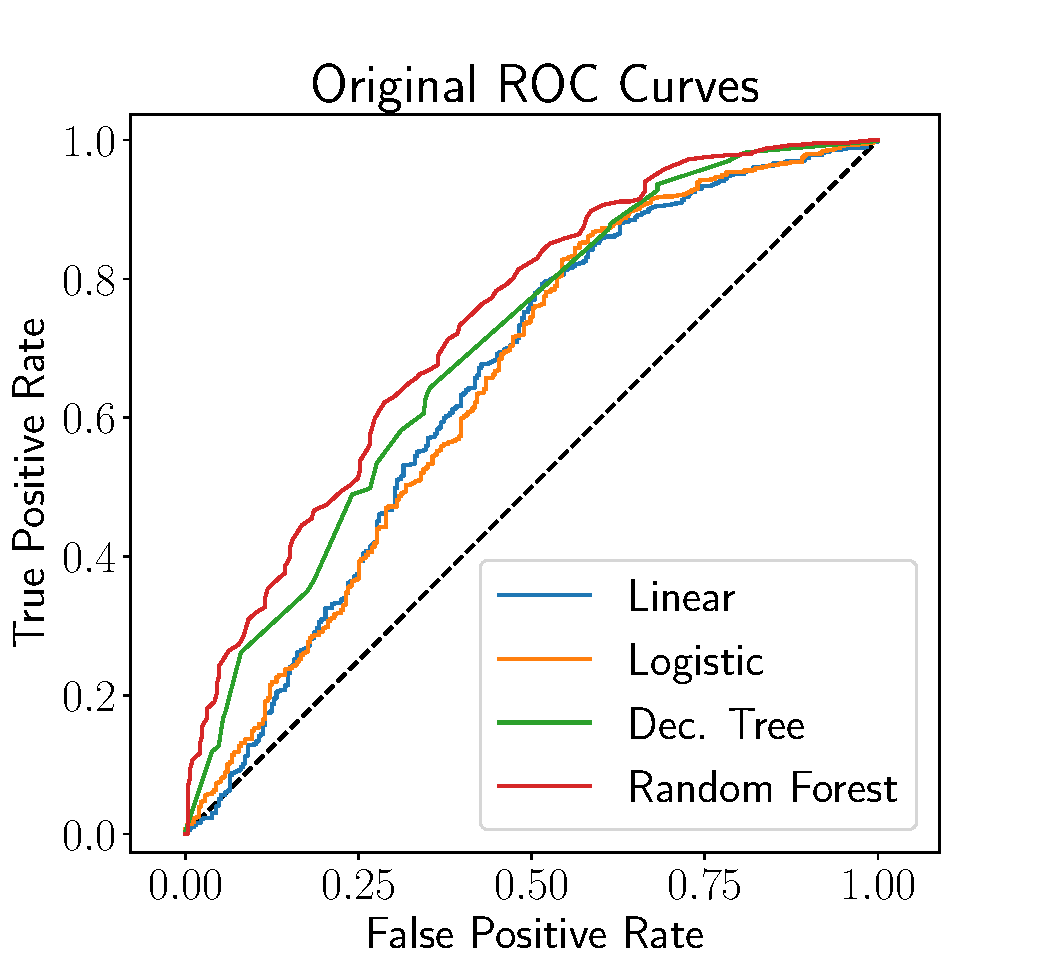
\includegraphics[width=1.0\linewidth]{oriROC.pdf}
    %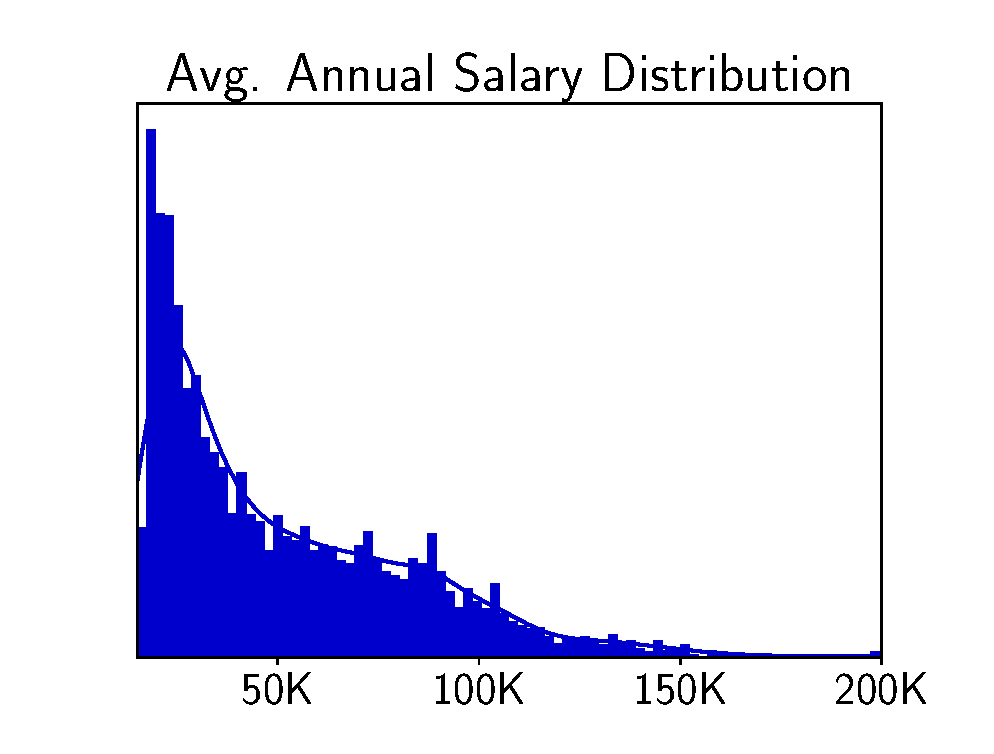
\includegraphics[trim={3cm 3cm 3cm 3cm}, clip,width=0.9\linewidth]{avgsal.eps}
	\caption{ROC curves for models trained on original variables}
	\label{fig:orgroc}
\end{figure}
%
Note that the performance of the linear and logistic regression models is very similar. 
In addition, the five level decision tree has stronger overall performance, and the 
random forest which is an ensemble model of such trees has the greatest performance overall.
However, additional complexity of the random forest raises the point that the simpler 
single decision tree may be preferred in practice since gains for the random forest 
are marginal.  Here the area under the ROC curve for the linear, decision tree an random forest 
is 65\%, 70\%, and 73\%, respectively.  

We next consider models evaluated on our extended features set; specifically, we add the 
rating PCA feature and the relative change in the employees salary after a job transition. 
The updated ROC curves are displayed in Figure \ref{fig:fullroc}
%
\begin{figure}[thb]
    \centering
	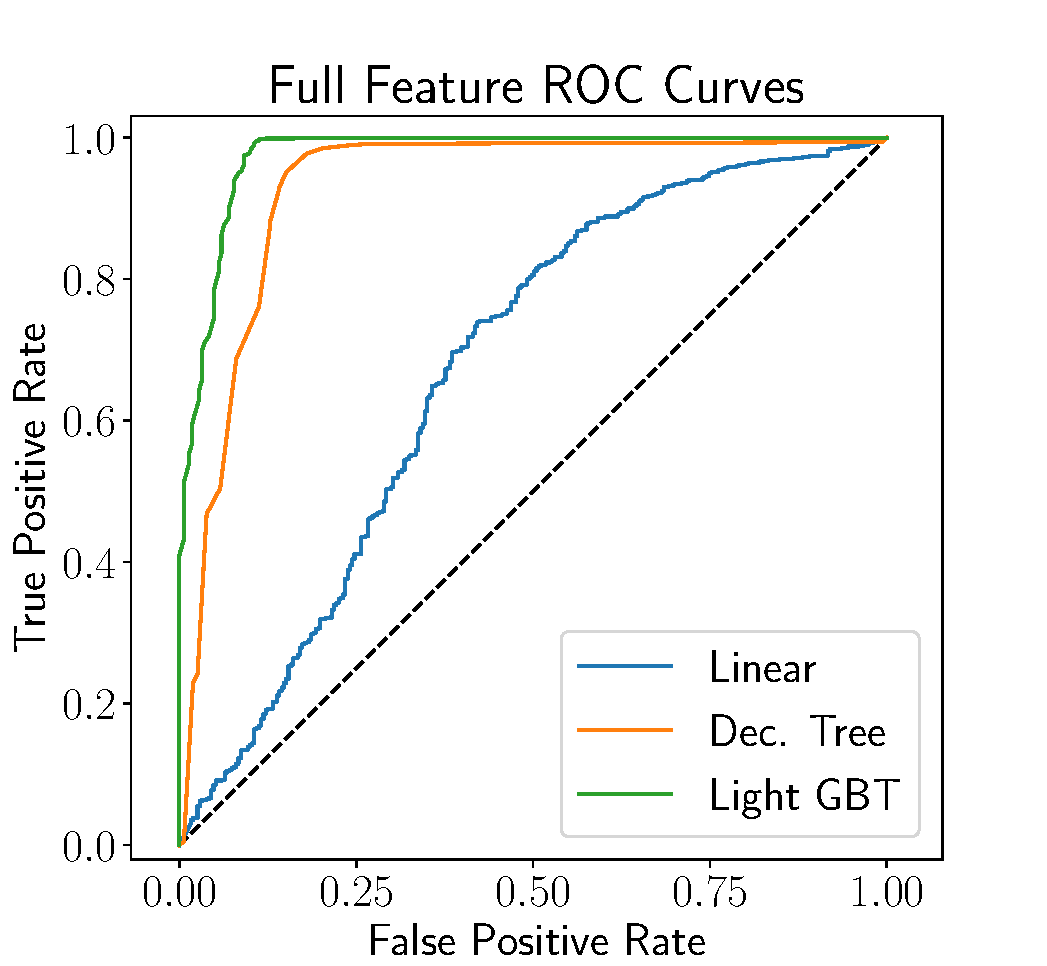
\includegraphics[width=1.0\linewidth]{fullROC.pdf}
    %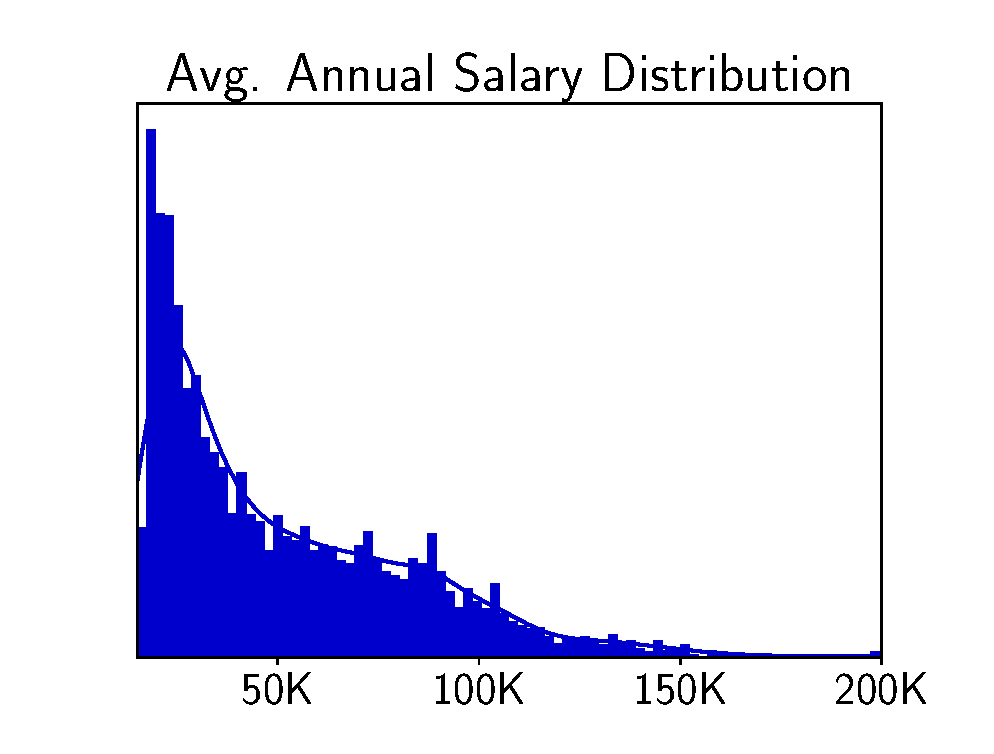
\includegraphics[trim={3cm 3cm 3cm 3cm}, clip,width=0.9\linewidth]{avgsal.eps}
	\caption{ROC curves for models trained on full feature set}
	\label{fig:fullroc}
\end{figure}
%
Here the areas under the ROC curves are given by 67\%, 58\%, 73\%, and 76\%, which demonstrates 
we are able to slightly improve the performance over the prior best model in the case of the 
light gradient boosted tree.  In addition, note that the linear regression model as very similar 
performance whereas the logistic regression model degrades in performance.  However the decision 
tree model also improves slightly.  Both examples provide a strong indicate that tree based models 
provide a good framework for the design of employee attrition classification. 

\section{Conclusions and Extensions} \label{consec}

In summary, we have obtained a dataset of employee job transitions generated from 
anonymously submitted resumes through Glassdoor's online portal. We found several 
insights upon an initial study of this data which provided an indication that 
compensation, company culture, and senior management performance play major 
roles in influencing an employee's job transition decision.  We then further investigated 
aspects of this data including generating an industry job transition table, identify 
which variables had the most significant changes in distribution for employees 
that stayed or left their current employers, and constructed ratings features 
based on a PCA study. We then applied several binary classification models 
to the employee attrition problem and found that tree based methods tended to 
offer the strongest performance.  In particular, in the case of the original 
variables specified in \cite{Smart2016}, simple decision trees offer strong 
performance whereas one of their extensions random forests provided a 
marginal increase at the addition of increased complexity.  Finally, we added 
in two new features including our original PCA based ratings feature
and the percentage salary increase of the job transition.  

We finally describe several ideas that we plan on pursing in future work.  First, 
we would like to construct a more extensions dataset of employee attrition data that goes
well beyond the 5550 job transitions considered in this article.  In particular, 
we hope to work with Glassdoor and/or LinkedIn to build a more extensive database of 
employee job transitions and associated company ratings. In addition, we would like to 
obtain company specific job transition information from LinkedIn which would permit 
more detailed attrition studies at the company and industry level to further 
the work of \cite{Bennet1993}.  In addition factors such as employee 
engagement and absence are known to have a strong connection with employee attrition 
\cite{Kumar2015,Mitra1992}.  Lastly, we 
note that if one wishes to examine the attrition problem in the greatest detail 
possible, then one would have to partner with firm to obtain specific detailed 
internal attrition records.  One could then develop company specific models, 
assuming sufficient data exists, that may be able to further extract information 
related to nuanced attrition patterns for that particular company.  The results 
may then be merged with verbal information gathered at exit interviews and 
human resource staff expertise to establish an attrition prevention plan. 

\textbf{Acknowledgements:} The authors would like to acknowledge Andrew Chamberlain, 
Chief Economist at Glassdoor, for sharing the job transition dataset that served 
as the data source for this study. 

% if added before the last page, this command can help balancing columns
%\addtolength{\textheight}{-.2cm} 

%Bibliography 
\bibliographystyle{ieeetr}
\bibliography{sample}

%\begin{enumerate}
%    \item how does salary increase compare with internal vs external transition? 
%    \item Founding date vs tenure
%    \item Let's focus on Leaving a company, not just different role in same company 
    %\item Look at rankings from old company to new one; what can we say overall about 
    %     the characteristics of these companies?  What factors did we see the most signi
    %     change in? Make scatter plots/hists here 
%    \item job title transition? progression ... Markov chain? 
%    \item What other summary statistics are relevant that go beyond what is already in 
%          the Glassdoor article? 
%    \item Do a brief literature review.  What has been done in this area already?
%          Summarize Glassdoor as part of this ... describe the uniqueness of this dataset. 
%          Mention it would be of interest to expand ... mine LinkedIn as well to do a 
%          more thorough study later. 
%    \item do reasons vary by length of job??? 
%    \item Look at people who made a major change (e.g. shifted geographic regions. ... more than 500 miles 
%          away ... is motivation any different for these people?)
%    \item Look at how old vs new ranking variable scatter plots differ from the y=x line, 
%        e.g. if employees change, which variables to we find also change significantly?  
%          Do some change always in the upwards direction? Linear reg. essentially tries 
%          to understand to what extent is this line differs from 1, e.g. if it is 1 for 
%          a given variable, then this variable has no influence ... can we develop a 
%          better variable influence measure here? 
%    \item Look at people who switched industries ... any different motivation here? 
%    \item One interesting feature is that employees seldom seem to stay at a company that has the 
%          same size as their old one.  Lots of shirts from large to small or vice versa.  Perhaps 
%          make this more quantitative? 
%    \item  check if job-len corresponds to start,end date difference 
%    \item Any info associated with geographic studies?  Large vs small cities? 
%    \item  patterns that stem from either age or employment tenure? 
%    \item binary model classifer, ROC curve etc. 
%    \item impl their original regression model ... test 
%    \item  industry specific studies 
%    \item Distribution of dates that changes were made ... do we see a pattern on times of the 
%          year that moves occurred 
%    \item explore patterns between old and new firms using year founded 
%\end{enumerate}

\end{document}


\end{document}
